\documentclass[hyperref={bookmarks=false},aspectratio=169]{beamer}
\usepackage{hyperref,ragged2e,amsmath,amssymb,url,bm}
\usepackage{graphicx,booktabs,array}
\usepackage{tikz}
\usetikzlibrary{arrows.meta,positioning,calc,shapes.geometric,decorations.pathreplacing,matrix}
\graphicspath{{crops/}}
\usetheme{Goettingen}
% --- Paleta: azul profundo, dorado y papiro crema ---
\definecolor{azul}{HTML}{15437C}
\definecolor{azuloscuro}{HTML}{0B1F3A}
\definecolor{celeste}{HTML}{5694D6}
\definecolor{dorado}{RGB}{196,154,60}
\definecolor{papiro}{RGB}{246,239,220}
\definecolor{gris}{RGB}{70,78,96}
\setbeamercolor{structure}{fg=azul}
\setbeamertemplate{sidebar canvas right}[vertical shading][top=azul,bottom=azuloscuro]
\setbeamercolor{title in sidebar}{fg=dorado}
\setbeamercolor{author in sidebar}{fg=papiro}
\setbeamercolor{section in sidebar}{fg=papiro}
\setbeamercolor{section in sidebar shaded}{fg=dorado!70!papiro}
\setbeamercolor{subsection in sidebar}{fg=papiro}
\setbeamercolor{subsection in sidebar shaded}{fg=dorado!70!papiro}
\let\raggedright\justifying
\setlength{\RaggedRightRightskip}{0pt plus 1fil}
\setbeamertemplate{background canvas}{
\includegraphics[width=\paperwidth,height=\paperheight]{papiro.jpg}}
\setbeamercolor{normal text}{fg=black!88!azuloscuro}
\setbeamercolor{frametitle}{fg=azul}
\setbeamerfont{frametitle}{series=\bfseries}
\setbeamertemplate{section in toc shaded}{\leavevmode{\color{gris}\inserttocsection}\par}
\setbeamercolor{title}{fg=azul}
\setbeamercolor{subtitle}{fg=gris}
\setbeamercolor{item projected}{bg=azul,fg=papiro}
\setbeamertemplate{itemize item}{\small\textcolor{dorado}{$\blacktriangleright$}}
\setbeamertemplate{navigation symbols}{}
% --- Español + hebreo + griego (XeLaTeX) ---
\usepackage[bidi=default]{babel}
\babelprovide[import,main]{spanish}
\babelprovide[import]{hebrew}
\babelprovide[import]{ancientgreek}
\babelfont[hebrew]{sf}[Path=fonts/, BoldFont=NotoHebrewSans-700.ttf]{NotoHebrewSans-400.ttf}
\babelfont[hebrew]{rm}[Path=fonts/, BoldFont=NotoHebrewSans-700.ttf]{NotoHebrewSans-400.ttf}
\babelfont[ancientgreek]{sf}[Path=fonts/]{GFSPorson.otf}
\babelfont[ancientgreek]{rm}[Path=fonts/]{GFSPorson.otf}
\newcommand{\heb}[1]{\mbox{\foreignlanguage{hebrew}{#1}}}
\newcommand{\grc}[1]{\foreignlanguage{ancientgreek}{#1}}
\newcommand{\SENOR}{S{\fontsize{0.78em}{1em}\selectfont EÑOR}}
% --- Citas (cuadro de un solo color), imágenes, referencias ---
\usepackage[most]{tcolorbox}
\newtcolorbox{cita}[1][]{enhanced, colback=azul!7!papiro, opacityback=0.85, colframe=azul,
  boxrule=0pt, leftrule=2.5pt, arc=0pt, left=6pt, right=6pt, top=4pt, bottom=4pt,
  before skip=4pt, after skip=6pt, fontupper=\small\itshape, #1}
\newcommand{\fuente}[1]{\par\hfill{\upshape\bfseries\footnotesize\textcolor{azul}{#1}}}
\makeatletter
\newcommand{\fotolado}[2]{%
  \begin{tikzpicture}[remember picture,overlay]
    \node[anchor=north east,inner sep=0pt] (foto) at ([xshift=-\beamer@sidebarwidth]current page.north east)
      {\includegraphics[height=\paperheight]{#1}};
    \node[anchor=south east,inner sep=2pt,text=papiro,fill=azuloscuro,fill opacity=0.6,text opacity=1,
      font=\fontsize{4.5}{5.5}\selectfont,align=right,text width=4.2cm] at ([xshift=-3pt,yshift=3pt]foto.south east)
      {\textit{Nota.} #2};
  \end{tikzpicture}}
\makeatother
\newcommand{\refapa}[1]{\par{\RaggedRight\hangindent=1.2em\hangafter=1\noindent #1\par}\vspace{3pt}}
\usepackage{xurl}\urlstyle{same}
\newcommand{\destacar}[1]{\textbf{\textcolor{azul}{#1}}}
\newcommand{\precision}[1]{{\footnotesize\color{gris}\textbf{Precisión:} #1}}
\tikzset{caja/.style={draw=azul,line width=0.8pt,fill=papiro,fill opacity=0.92,text opacity=1,rounded corners=3pt,inner sep=5pt,font=\scriptsize}}
\title[La preexistencia]{\bfseries{La preexistencia de Dios}}
\subtitle{``YO SOY EL QUE SOY'' (Éx 3:14)}
\author{}\institute{}\date{}
\titlegraphic{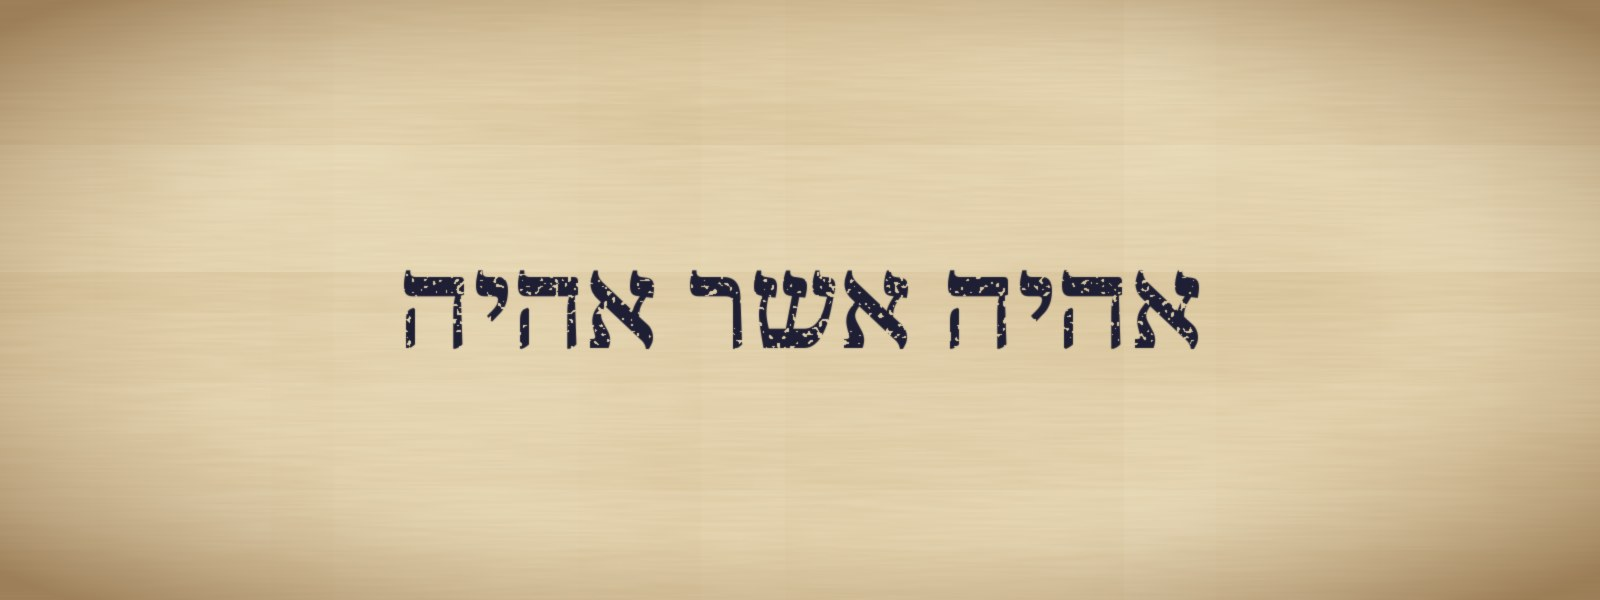
\includegraphics[width=0.80\linewidth,height=0.36\textheight,keepaspectratio]{portada.jpg}\\[-1pt]
  {\fontsize{5}{6}\selectfont\color{gris}\textit{Nota.} Elaboración propia: Éx 3:14 en texto hebreo consonántico (BHS).}}
\begin{document}
\frame{\titlepage}

\begin{frame}\frametitle{Contenidos}\tableofcontents\end{frame}

% ------------------------------------------------------------------
\section{Antes que todo}

\begin{frame}{¿Qué había antes de todo?}
\begin{columns}[c,onlytextwidth]
\begin{column}{0.50\textwidth}
\begin{tcolorbox}[colback=papiro,colframe=dorado,boxrule=1.2pt,arc=3pt]
\centering\small \destacar{Dios existe por sí mismo y no depende de nada.}
\end{tcolorbox}
\small\RaggedRight Toda criatura tiene un ``antes'': los montes, el sol, el mar, el ser humano. Dios no. La Escritura responde a la pregunta más antigua con un Nombre.
\end{column}
\begin{column}{0.48\textwidth}
\begin{center}\heb{בְּטֶרֶם הָרִים יֻלָּדוּ וַתְּחוֹלֵל אֶרֶץ וְתֵבֵל}\\[1pt]\heb{וּמֵעוֹלָם עַד־עוֹלָם אַתָּה אֵל}\end{center}
\begin{cita}Antes que naciesen los montes Y formases la tierra y el mundo, Desde el siglo y hasta el siglo, tú eres Dios.\fuente{(Sal 90:2, RVR1960)}\end{cita}
\scriptsize El salmista no dice ``tú eras'': \heb{אַתָּה אֵל} (\emph{atá El}) no tiene verbo, como si Dios no tuviera pasado.
\end{column}
\end{columns}
\end{frame}

\begin{frame}{Tres rasgos de un mismo atributo}
\centering
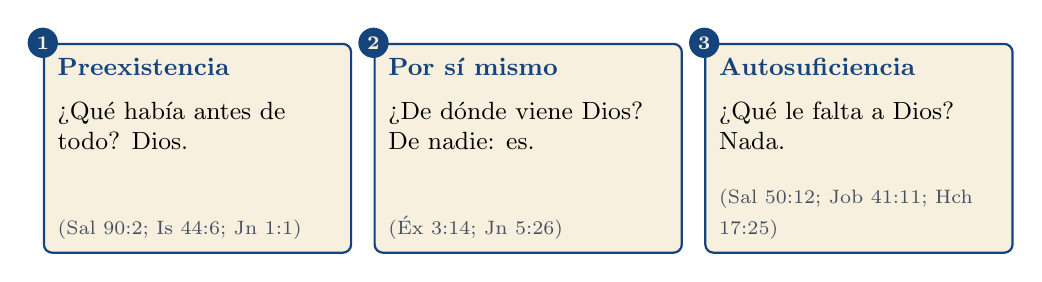
\begin{tikzpicture}
 \foreach \x/\n/\t/\d/\r in {0/1/{Preexistencia}/{¿Qué había antes de todo? Dios.}/{Sal 90:2; Is 44:6; Jn 1:1},
   4.2/2/{Por sí mismo}/{¿De dónde viene Dios? De nadie: es.}/{Éx 3:14; Jn 5:26},
   8.4/3/{Autosuficiencia}/{¿Qué le falta a Dios? Nada.}/{Sal 50:12; Job 41:11; Hch 17:25}}{
  \node[caja,anchor=north] (b\n) at (\x,0) {\parbox[t][2.3cm][t]{3.55cm}{\RaggedRight
    {\small\textbf{\textcolor{azul}{\t}}}\\[5pt]\small \d\par\vfill{\scriptsize\color{gris}(\r)}}};
  \node[circle,fill=azul,text=papiro,font=\scriptsize\bfseries,inner sep=1.6pt] at (b\n.north west) {\n};}
\end{tikzpicture}\par\medskip
\begin{cita}Mas alábese en esto el que se hubiere de alabar: en entenderme y conocerme, que yo soy \SENOR{}\ldots\fuente{(Jer 9:24 [9:23], RVR1960)}\end{cita}
\scriptsize Conocer a alguien empieza por saber de dónde viene. Con Dios la respuesta es única: no viene de nadie, y todo viene de él.\par
\precision{la definición es la de tu material; la teología clásica la llama \emph{aseidad} (latín \emph{a se}, ``por sí mismo'') o independencia de Dios (Berkhof, 1938; Grudem, 2007).}
\end{frame}

% ------------------------------------------------------------------
\section{Éxodo 3}

\begin{frame}{Una zarza que no se consume}
\begin{columns}[t,onlytextwidth]
\begin{column}{0.52\textwidth}
\begin{center}\heb{וְהִנֵּה הַסְּנֶה בֹּעֵר בָּאֵשׁ וְהַסְּנֶה אֵינֶנּוּ אֻכָּל}\end{center}
\begin{cita}Y se le apareció el Angel de \SENOR{} en una llama de fuego en medio de una zarza; y él miró, y vio que la zarza ardía en fuego, y la zarza no se consumía.\fuente{(Éx 3:2, RVR1960)}\end{cita}
\end{column}
\begin{column}{0.46\textwidth}\small
\begin{itemize}
\item Todo fuego depende de algo: necesita leña y se apaga cuando la consume.
\item Este fuego arde y la zarza sigue entera. Moisés se acerca a ver ``por qué causa la zarza no se quema'' (3:3).
\item Desde ese fuego Dios dice su Nombre.
\end{itemize}
\precision{leer la zarza como imagen de un Dios que no depende de combustible es lectura propia de esta serie; la tradición judía la leyó también como figura de Israel, que sufre en Egipto sin ser destruido.}
\end{column}
\end{columns}
\end{frame}

\begin{frame}{Texto ancla: Éx 3:13--15}
\fotolado{panel_exodo3.jpg}{Elaboración propia: Éx 3:14 en texto hebreo consonántico (BHS).}
\begin{columns}[c,onlytextwidth]
\begin{column}{0.58\textwidth}
\begin{cita}Dijo Moisés a Dios: He aquí que llego yo a los hijos de Israel, y les digo: El Dios de vuestros padres me ha enviado a vosotros. Si ellos me preguntaren: ¿Cuál es su nombre?, ¿qué les responderé? Y respondió Dios a Moisés: YO SOY EL QUE SOY. Y dijo: Así dirás a los hijos de Israel: YO SOY me envió a vosotros.\fuente{(Éx 3:13--14, RVR1960)}\end{cita}
\begin{cita}\ldots{} Este es mi nombre para siempre; con él se me recordará por todos los siglos.\fuente{(Éx 3:15, RVR1960)}\end{cita}
\end{column}
\begin{column}{0.40\textwidth}\end{column}
\end{columns}
\end{frame}

\begin{frame}{Éx 3:14 en hebreo}
\begin{center}
\heb{וַיֹּאמֶר אֱלֹהִים אֶל־מֹשֶׁה אֶהְיֶה אֲשֶׁר אֶהְיֶה}\\[2pt]
\heb{וַיֹּאמֶר כֹּה תֹאמַר לִבְנֵי יִשְׂרָאֵל אֶהְיֶה שְׁלָחַנִי אֲלֵיכֶם}
\end{center}
\renewcommand{\arraystretch}{1.12}\scriptsize
\begin{tabular}{@{}>{\RaggedRight\arraybackslash}p{2.9cm}>{\RaggedRight\arraybackslash}p{1.2cm}>{\RaggedRight\arraybackslash}p{7.7cm}@{}}
\toprule
\textbf{Término} & \textbf{Raíz} & \textbf{Sentido} \\ \midrule
\heb{אֶהְיֶה} \emph{ehyeh} & \heb{היה} & imperfecto de \emph{hayá}, ``ser, existir, estar presente'': ``soy'', ``seré'' o ``estaré''. \\
\heb{אֲשֶׁר} \emph{asher} & --- & ``el que'': la fórmula se cierra sobre sí misma. Dios se define por Dios. \\
\heb{אֶהְיֶה שְׁלָחַנִי} & \heb{שׁלח} & ``\emph{Ehyeh} me envió'': el verbo se vuelve Nombre propio. \\
\grc{ἐγώ εἰμι ὁ ὤν} & \grc{εἰμί} & la LXX: ``Yo soy el que es''. \\
\heb{יהוה} (3:15) & \heb{היה}? & el Nombre en tercera persona: se escucha como ``Él es''. \\
\bottomrule
\end{tabular}\par\smallskip
\precision{``Yo soy el que soy'' (LXX, RVR1960) subraya el ser; ``Seré el que seré'' subraya la presencia, apoyada en 3:12, \heb{אֶהְיֶה עִמָּךְ}, ``yo estaré contigo'' (HALOT). El hebreo permite las dos; el contexto las une. El origen exacto de \heb{יהוה} se discute.}
\end{frame}

\begin{frame}{Ser y estar: Éx 3:12 y 3:14}
\centering
\begin{tikzpicture}[font=\small,node distance=1.1cm]
 \node[caja,text width=3.6cm,align=center,font=\small] (a) {\textbf{Éx 3:12}\\ \heb{כִּי־אֶהְיֶה עִמָּךְ}\\ ``yo \emph{estaré} contigo''};
 \node[draw=dorado,line width=1.6pt,fill=azul,text=papiro,rounded corners=3pt,text width=3.6cm,align=center,inner sep=6pt,right=of a] (b) {\textbf{Éx 3:14}\\ \heb{אֶהְיֶה אֲשֶׁר אֶהְיֶה}\\ ``YO \emph{SOY} EL QUE SOY''};
 \node[caja,text width=3.6cm,align=center,font=\small,right=of b] (c) {\textbf{Éx 3:7--8}\\ ``he descendido para librarlos''};
 \draw[-{Latex[length=3mm]},dorado,line width=1.4pt] (a)--(b);
 \draw[-{Latex[length=3mm]},dorado,line width=1.4pt] (b)--(c);
\end{tikzpicture}\par\bigskip
\small El Dios que \destacar{es} por sí mismo es el Dios que \destacar{está} con su siervo. El que no depende de nadie baja a librar a un pueblo que depende de todo.\par\medskip
\scriptsize El v. 15 ata el Nombre a Abraham, Isaac y Jacob: el Dios que existía antes de los patriarcas es el que se unió a ellos con un pacto.
\end{frame}

% ------------------------------------------------------------------
\section{La palabra}

\begin{frame}{Decir ``antes'' de Dios}
\scriptsize\renewcommand{\arraystretch}{1.08}
\begin{tabular}{@{}>{\RaggedRight\arraybackslash}p{3.0cm}>{\RaggedRight\arraybackslash}p{0.7cm}>{\RaggedRight\arraybackslash}p{4.3cm}>{\RaggedRight\arraybackslash}p{3.6cm}@{}}
\toprule
\textbf{Expresión} & \textbf{Veces} & \textbf{Sentido (RVR1960)} & \textbf{Textos} \\ \midrule
\heb{אֶהְיֶה} \emph{ehyeh} & 51 & ``seré, estaré''; ``YO SOY'' & Éx 3:12, 14; Pr 8:30 \\
\heb{אֲנִי הוּא} \emph{ani hu} & 8 & ``yo soy'', ``yo mismo'' & Dt 32:39; Is 43:10, 13; 46:4 \\
\heb{בְּטֶרֶם} \emph{béterem} & 45 & ``antes que'' & Sal 90:2; Jer 1:5 \\
\heb{מִקֶּדֶם}; \heb{אֱלֹהֵי קֶדֶם} & 24; 1 & ``desde el principio''; ``el eterno Dios'' & Dt 33:27; Is 46:10; Hab 1:12 \\
\heb{רִאשׁוֹן} y \heb{אַחֲרוֹן} & 3 & ``el primero\ldots{} el postrero'' & Is 41:4; 44:6; 48:12 \\
\heb{מֵעוֹלָם עַד־עוֹלָם} & 6 & ``desde el siglo y hasta el siglo'' & Sal 90:2; Neh 9:5 \\ \midrule
\grc{πρὸ καταβολῆς κόσμου} & 3 & ``antes de la fundación del mundo'' & Jn 17:24; Ef 1:4; 1 P 1:20 \\
\grc{πρὸ χρόνων αἰωνίων} & 2 & ``antes de los tiempos de los siglos'' & 2 Ti 1:9; Tit 1:2 \\
\grc{πρὸ πάντων} & 1 & ``antes de todas las cosas'' & Col 1:17 \\
\grc{πρὶν Ἀβραὰμ γενέσθαι} & 1 & ``antes que Abraham fuese'' & Jn 8:58 \\
\grc{ἐγώ εἰμι} absoluto & 7 & ``yo soy'', sin predicado & Jn 8:24, 28, 58; 13:19; 18:5--8 \\
\grc{προγινώσκω}; \grc{πρόγνωσις} & 5; 2 & ``conocer antes''; ``anticipado conocimiento'' & Hch 2:23; Ro 8:29 \\
\grc{προσδέομαι} & 1 & ``necesitar de algo'' & Hch 17:25 \\
\bottomrule
\end{tabular}\par\smallskip
\precision{conteo propio (BHS y NA27 con Strong); verificar en e-Sword. ``Preexistencia'' no aparece en la Biblia: el hebreo lo dice con verbos, pronombres y adverbios de tiempo.}
\end{frame}

\begin{frame}{\emph{Ani hu}: ``Yo soy''}
\begin{columns}[t,onlytextwidth]
\begin{column}{0.54\textwidth}
\begin{center}\heb{כִּי־אֲנִי הוּא לְפָנַי לֹא־נוֹצַר אֵל וְאַחֲרַי לֹא יִהְיֶה}\end{center}
\begin{cita}Vosotros sois mis testigos, dice \SENOR, y mi siervo que yo escogí, para que me conozcáis y creáis, y entendáis que yo mismo soy; antes de mí no fue formado dios, ni lo será después de mí.\fuente{(Is 43:10, RVR1960)}\end{cita}
\begin{cita}Aun antes que hubiera día, yo era\ldots\fuente{(Is 43:13, RVR1960)}\end{cita}
\end{column}
\begin{column}{0.44\textwidth}\scriptsize
\begin{itemize}
\item \heb{אֲנִי הוּא}: ``yo (soy) él'', frase sin verbo. La LXX traduce \grc{ἐγώ εἰμι}.
\item \heb{לֹא־נוֹצַר}: ``no fue formado'', con \emph{yatsar}, el verbo del alfarero (Gn 2:7). Todo dios ``formado'' tiene un antes; Dios no.
\item Israel es ``testigo'' de este Dios: lo conoce y \emph{cree} (\heb{וְתַאֲמִינוּ}, raíz \emph{amán}).
\item Dt 32:39 e Isaías 40--48 usan la fórmula frente a los dioses que no existían antes ni existirán después.
\end{itemize}
\end{column}
\end{columns}
\end{frame}

\begin{frame}{Del Nombre a Jesús}
\centering
\begin{tikzpicture}[font=\small,node distance=0.9cm]
 \node[caja,text width=3.4cm,align=center,font=\small] (h) {\textbf{Hebreo}\\ \heb{אֶהְיֶה} (Éx 3:14)\\ \heb{אֲנִי הוּא} (Dt 32:39; Is 43:10)};
 \node[caja,text width=3.4cm,align=center,font=\small,right=of h] (l) {\textbf{Septuaginta}\\ \grc{ἐγώ εἰμι ὁ ὤν}\\ \grc{ἐγώ εἰμι}};
 \node[draw=dorado,line width=1.6pt,fill=azul,text=papiro,rounded corners=3pt,text width=3.4cm,align=center,inner sep=6pt,right=of l] (p) {\textbf{Jesús}\\ \grc{πρὶν Ἀβραὰμ γενέσθαι}\\ \grc{ἐγὼ εἰμί} (Jn 8:58)};
 \draw[-{Latex[length=3mm]},dorado,line width=1.4pt] (h)--(l);
 \draw[-{Latex[length=3mm]},dorado,line width=1.4pt] (l)--(p);
\end{tikzpicture}\par\medskip
{\scriptsize\itshape\color{gris} La misma fórmula recorre el Nombre de la zarza, la Septuaginta de Isaías y la boca de Jesús.}
\end{frame}

\begin{frame}{\emph{Béterem}: conocido antes de existir}
\begin{columns}[t,onlytextwidth]
\begin{column}{0.52\textwidth}
\begin{center}\heb{בְּטֶרֶם אֶצָּרְךָ בַבֶּטֶן יְדַעְתִּיךָ}\end{center}
\begin{cita}Antes que te formase en el vientre te conocí, y antes que nacieses te santifiqué, te di por profeta a las naciones.\fuente{(Jer 1:5, RVR1960)}\end{cita}
\end{column}
\begin{column}{0.46\textwidth}\scriptsize\renewcommand{\arraystretch}{1.12}
\begin{tabular}{@{}>{\RaggedRight\arraybackslash}p{1.5cm}>{\RaggedRight\arraybackslash}p{3.9cm}@{}}
\toprule
\heb{בְּטֶרֶם} & ``antes que'': el conocimiento de Dios precede a la existencia del profeta. \\
\heb{אֶצָּרְךָ} & ``te formase'': \emph{yatsar}, el alfarero. \\
\heb{יְדַעְתִּיךָ} & ``te conocí'': conocer es relación y elección (Gn 18:19; Am 3:2). \\
\bottomrule
\end{tabular}\par\medskip
\small El libro que dice ``conocerme'' (Jer 9:24) empieza diciendo que Dios \destacar{conoció primero}. Aquí la preexistencia toca la \destacar{presciencia}: Dios conoce antes porque es antes.
\end{column}
\end{columns}
\end{frame}

\begin{frame}{\emph{Miqqédem}: desde siempre}
\begin{columns}[t,onlytextwidth]
\begin{column}{0.50\textwidth}
\begin{center}\heb{הֲלוֹא אַתָּה מִקֶּדֶם יְהוָה אֱלֹהַי קְדֹשִׁי לֹא נָמוּת}\end{center}
\begin{cita}¿No eres tú desde el principio, oh \SENOR, Dios mío, Santo mío? No moriremos\ldots\fuente{(Hab 1:12, RVR1960)}\end{cita}
\scriptsize \heb{קֶדֶם} (\emph{qédem}): lo que está delante; el oriente y lo antiguo. Moisés llama a Dios \heb{אֱלֹהֵי קֶדֶם}, ``el eterno Dios'' (Dt 33:27). Habacuc saca la consecuencia: si Dios es desde el principio, su pueblo ``no morirá''.
\end{column}
\begin{column}{0.48\textwidth}
\begin{center}\heb{מְעֹנָה אֱלֹהֵי קֶדֶם וּמִתַּחַת זְרֹעֹת עוֹלָם}\end{center}
\begin{cita}El eterno Dios es tu refugio, Y acá abajo los brazos eternos\ldots\fuente{(Dt 33:27, RVR1960)}\end{cita}
\scriptsize \heb{אֱלֹהֵי קֶדֶם} (\emph{Elohé qédem}): ``el Dios de antes''. La última bendición de Moisés pone el refugio de Israel en el Dios que estaba antes de todo, y sus brazos debajo.
\end{column}
\end{columns}
\end{frame}

\begin{frame}{``¿Quién me ha dado a mí primero?''}
\begin{columns}[t,onlytextwidth]
\begin{column}{0.52\textwidth}
\begin{center}\heb{מִי הִקְדִּימַנִי וַאֲשַׁלֵּם תַּחַת כָּל־הַשָּׁמַיִם לִי־הוּא}\end{center}
\begin{cita}¿Quién me ha dado a mí primero, para que yo restituya? Todo lo que hay debajo del cielo es mío.\fuente{(Job 41:11 [41:3], RVR1960)}\end{cita}
\begin{cita}Si yo tuviese hambre, no te lo diría a ti; Porque mío es el mundo y su plenitud.\fuente{(Sal 50:12, RVR1960)}\end{cita}
\end{column}
\begin{column}{0.46\textwidth}\scriptsize
\begin{itemize}
\item \heb{הִקְדִּימַנִי} (\emph{hiqdimani}): ``se me adelantó'', ``me dio primero''; hifil de la raíz de \emph{qédem}.
\item Dios es \emph{qédem} (antes); por eso nadie se le \emph{adelanta} (\emph{hiqdim}) para dejarlo en deuda.
\item \heb{אִם־אֶרְעַב}: ``si tuviera hambre'', condición irreal. Los sacrificios no alimentan a Dios (50:13).
\item Pablo cita Job 41:11 en Ro 11:35.
\end{itemize}
\end{column}
\end{columns}
\end{frame}

% ------------------------------------------------------------------
\section{El Nombre}

\begin{frame}{``Yo soy el primero, y yo soy el postrero''}
\begin{columns}[t,onlytextwidth]
\begin{column}{0.52\textwidth}
\begin{center}\heb{אֲנִי רִאשׁוֹן וַאֲנִי אַחֲרוֹן וּמִבַּלְעָדַי אֵין אֱלֹהִים}\end{center}
\begin{cita}Así dice \SENOR{} Rey de Israel, y su Redentor, \SENOR{} de los ejércitos: Yo soy el primero, y yo soy el postrero, y fuera de mí no hay Dios.\fuente{(Is 44:6, RVR1960)}\end{cita}
\scriptsize También Is 41:4 y 48:12, siempre frente a los ídolos y al exilio.
\end{column}
\begin{column}{0.46\textwidth}\scriptsize\renewcommand{\arraystretch}{1.12}
\begin{tabular}{@{}>{\RaggedRight\arraybackslash}p{1.7cm}>{\RaggedRight\arraybackslash}p{3.7cm}@{}}
\toprule
\heb{רִאשׁוֹן} & ``primero'', de \emph{rosh}, ``cabeza''; misma raíz que \emph{reshit}, ``principio'' (Gn 1:1). \\
\heb{אַחֲרוֹן} & ``último'': el que queda cuando todo pasó. \\
\heb{מִבַּלְעָדַי} & ``fuera de mí'': título exclusivo. \\
\heb{גֹּאֲלוֹ} & ``su Redentor'': el Primero es el pariente que rescata. \\
\bottomrule
\end{tabular}\par\medskip
\small No es el primero de una lista: es el primero porque \destacar{todo viene de él}, y el último porque nada lo sobrevive.
\end{column}
\end{columns}
\end{frame}

\begin{frame}{El Alfa y la Omega}
\centering
\begin{tikzpicture}[font=\small,node distance=0.8cm]
 \node[caja,text width=3.3cm,align=center,font=\small] (a) {\textbf{Is 44:6}\\ \heb{אֲנִי רִאשׁוֹן וַאֲנִי אַחֲרוֹן}\\ el \SENOR};
 \node[caja,text width=3.3cm,align=center,font=\small,right=of a] (b) {\textbf{Ap 1:8}\\ \grc{τὸ ἄλφα καὶ τὸ ὦ}\\ ``dice el Señor''};
 \node[draw=dorado,line width=1.6pt,fill=azul,text=papiro,rounded corners=3pt,text width=3.3cm,align=center,inner sep=6pt,right=of b] (c) {\textbf{Ap 1:17; 22:13}\\ \grc{ὁ πρῶτος καὶ ὁ ἔσχατος}\\ Jesús};
 \draw[-{Latex[length=3mm]},dorado,line width=1.4pt] (a)--(b);
 \draw[-{Latex[length=3mm]},dorado,line width=1.4pt] (b)--(c);
\end{tikzpicture}\par\medskip
\begin{columns}[t,onlytextwidth]
\begin{column}{0.49\textwidth}\scriptsize
El título exclusivo del \SENOR{} (``fuera de mí no hay Dios'') pasa sin cambios a Jesús.\par\smallskip
\precision{el análisis del título en Ap es de Bauckham (1993). Éx 3:14, el Nombre de la zarza, se estudiará también en el capítulo sobre el Dios eterno.}
\end{column}
\begin{column}{0.49\textwidth}
\begin{cita}\ldots{} él que es el principio, el primogénito de entre los muertos, para que en todo tenga la preeminencia.\fuente{(Col 1:18, RVR1960)}\end{cita}
\scriptsize Pablo: \grc{ὅς ἐστιν ἀρχή}. Y el ``nombre que es sobre todo nombre'' (Flp 2:9--11 = Is 45:23).
\end{column}
\end{columns}
\end{frame}

% ------------------------------------------------------------------
\section{Definición}

\begin{frame}{Definición}
\begin{tcolorbox}[colback=papiro,colframe=azul,boxrule=1pt,arc=3pt,fonttitle=\bfseries,title=La preexistencia de Dios]
\small Es la perfección eterna por la cual Dios existe antes de todas las cosas, por sí mismo y sin depender de nada. Nadie le dio el ser, nadie lo sostiene y nada le falta; todo lo que existe recibe de él vida, aliento y todas las cosas (Éx 3:14; Sal 90:2; Hch 17:24--25).
\end{tcolorbox}
\scriptsize\renewcommand{\arraystretch}{1.1}
\begin{tabular}{@{}>{\RaggedRight\arraybackslash}p{2.6cm}>{\RaggedRight\arraybackslash}p{5.4cm}>{\RaggedRight\arraybackslash}p{3.6cm}@{}}
\toprule
\textbf{Rasgo} & \textbf{Qué afirma} & \textbf{Textos} \\ \midrule
Antes de todo & cuando nada existía, Dios era & Sal 90:2; Is 43:10; Jn 1:1 \\
Por sí mismo & su ser no viene de otro & Éx 3:14; Jn 5:26 \\
Sin necesidad & no necesita alimento, templo ni ayuda & Sal 50:12; Hch 17:25 \\
Sin deuda & nadie le dio primero & Job 41:11; Ro 11:35 \\
Fuente de todo & todo recibe de él el ser & Neh 9:6; Ro 11:36; Ap 4:11 \\
Con un plan previo & conoce y decide antes de crear & Is 46:10; Jer 1:5; Ef 1:4 \\
\bottomrule
\end{tabular}
\end{frame}

\begin{frame}{Clasificación}
\begin{columns}[c,onlytextwidth]
\begin{column}{0.48\textwidth}
\begin{tcolorbox}[colback=azul!8!papiro,colframe=azul,boxrule=0.8pt,arc=3pt,title=Ser,fonttitle=\bfseries\small]
\small Responde a ``¿qué es Dios?''. Abre la serie porque los demás atributos la suponen: un Dios dependiente tendría santidad, poder o amor \emph{prestados}.
\end{tcolorbox}
\end{column}
\begin{column}{0.48\textwidth}
\begin{tcolorbox}[colback=dorado!12,colframe=dorado,boxrule=0.8pt,arc=3pt,title=Incomunicable,fonttitle=\bfseries\small,coltitle=azuloscuro]
\small Ninguna criatura existe por sí misma. Solo el Hijo tiene ``vida en sí mismo'', porque el Padre se la dio (Jn 5:26).
\end{tcolorbox}
\end{column}
\end{columns}\medskip
\begin{cita}Porque como el Padre tiene vida en sí mismo, así también ha dado al Hijo el tener vida en sí mismo.\fuente{(Jn 5:26, RVR1960)}\end{cita}
\end{frame}

\begin{frame}{Preexistencia, eternidad y presciencia}
\centering
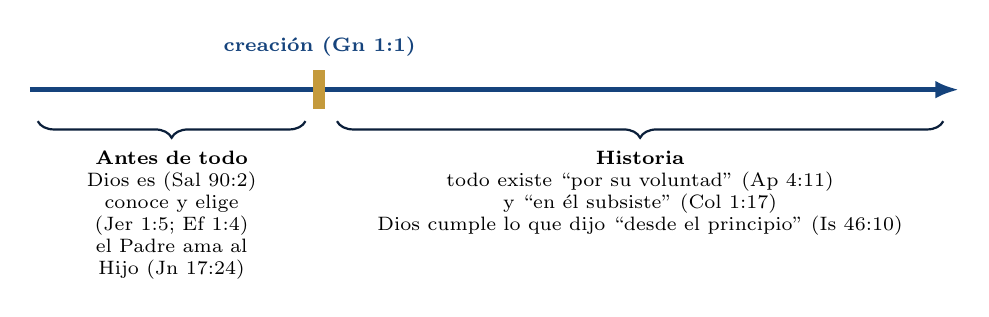
\begin{tikzpicture}[font=\small]
 \draw[line width=1.6pt,azul,-{Latex[length=3mm]}] (0,0) -- (11.8,0);
 \fill[dorado] (3.6,-0.25) rectangle (3.75,0.25);
 \node[font=\scriptsize\bfseries,text=azul,above] at (3.68,0.3) {creación (Gn 1:1)};
 \draw[decorate,decoration={brace,amplitude=6pt,mirror},line width=0.8pt,azuloscuro] (0.1,-0.4) -- (3.5,-0.4);
 \node[text width=3.4cm,align=center,font=\scriptsize,below] at (1.8,-0.65) {\textbf{Antes de todo}\\ Dios es (Sal 90:2)\\ conoce y elige (Jer 1:5; Ef 1:4)\\ el Padre ama al Hijo (Jn 17:24)};
 \draw[decorate,decoration={brace,amplitude=6pt,mirror},line width=0.8pt,azuloscuro] (3.9,-0.4) -- (11.6,-0.4);
 \node[text width=7.2cm,align=center,font=\scriptsize,below] at (7.75,-0.65) {\textbf{Historia}\\ todo existe ``por su voluntad'' (Ap 4:11)\\ y ``en él subsiste'' (Col 1:17)\\ Dios cumple lo que dijo ``desde el principio'' (Is 46:10)};
\end{tikzpicture}\par\medskip
\begin{columns}[t,onlytextwidth]
\begin{column}{0.49\textwidth}\scriptsize
\textbf{Eternidad:} Dios no tiene principio ni fin, y el tiempo no lo mide (Sal 90:4; 102:27). Tendrá su propio capítulo. \textbf{Preexistencia} mira hacia atrás desde la creación: antes del primer día, Dios ya era.
\end{column}
\begin{column}{0.49\textwidth}\scriptsize
\textbf{Presciencia:} si Dios era antes de todo, su conocimiento y su consejo también. ``Anuncio lo por venir desde el principio\ldots{} Mi consejo permanecerá'' (Is 46:10).
\end{column}
\end{columns}
\end{frame}

% ------------------------------------------------------------------
\section{Teología}

\begin{frame}{Antes de ``En el principio'': un Dios completo}
\begin{columns}[t,onlytextwidth]
\begin{column}{0.52\textwidth}\small
La Biblia no empieza explicando a Dios, sino con Dios: ``En el principio creó Dios'' (Gn 1:1). Antes de ese principio no había cielo, ni tierra, ni ángeles; solo Dios. Y ese Dios no estaba incompleto, esperando algo que la creación le diera.\par\medskip
\begin{tcolorbox}[colback=papiro,colframe=dorado,boxrule=1pt,arc=3pt]
\centering\small Dios estaba ``completo, autosuficiente, satisfecho de Sí mismo y sin necesidad de nada''.\par
{\scriptsize\color{gris}(Pink, 2020, cap. 1)}
\end{tcolorbox}
\end{column}
\begin{column}{0.46\textwidth}\scriptsize
De ahí se sigue, primero, que \textbf{crear fue libre}: si el universo le hubiera sido necesario, habría existido siempre; Dios lo hizo ``según el designio de su voluntad'' (Ef 1:11), y nada se agregó a su ser (Mal 3:6).\par\smallskip
Se sigue también que \textbf{nada le añade}, ni siquiera la adoración: su Nombre está ``alto sobre toda bendición y alabanza'' (Neh 9:5), y Eliú pregunta: ``Si fueres justo, ¿qué le darás a él?'' (Job 35:7).\par\smallskip
Por eso, en fin, \textbf{nadie lo pone en deuda}: ``¿O quién le dio a él primero, para que le fuese recompensado?'' (Ro 11:35). Lo que la criatura da a Dios ya era de él.
\end{column}
\end{columns}
\end{frame}

\begin{frame}{``Como la gota de agua que cae del cubo''}
\begin{columns}[c,onlytextwidth]
\begin{column}{0.55\textwidth}
\begin{cita}He aquí que las naciones le son como la gota de agua que cae del cubo, y como menudo polvo en las balanzas le son estimadas\ldots{} Como nada son todas las naciones delante de él; y en su comparación serán estimadas en menos que nada, y que lo que no es. ¿A qué, pues, haréis semejante a Dios, o qué imagen le compondréis?\fuente{(Is 40:15, 17--18, RVR1960)}\end{cita}
\end{column}
\begin{column}{0.43\textwidth}
\scriptsize Isaías no rebaja a las naciones para despreciarlas, sino para medir a Dios: todo lo que existe pesa ante él lo que una gota. El que no necesita nada es el que lo sostiene todo.\par\smallskip
\begin{tcolorbox}[colback=azul,colframe=dorado,boxrule=1.2pt,arc=3pt,coltext=papiro]
\centering\small Dios ``lo sostiene todo, pero es independiente de todo. Él da a todos, pero de ninguno se enriquece''.\par{\scriptsize(Pink, 2020, cap. 1)}
\end{tcolorbox}
\scriptsize Pablo lo nombra así: el ``solo Soberano'', ``el único que tiene inmortalidad'' (1 Ti 6:15--16).\par\smallskip
\precision{Sal 16:2 se ha leído como palabras de Cristo según la RV1909 (``mi bien a ti no aprovecha''; Pink, 2020, cap. 1); la RVR1960 y el hebreo dicen otra cosa, por eso no se usa aquí.}
\end{column}
\end{columns}
\end{frame}

\begin{frame}{La presciencia mira a personas}
\begin{columns}[t,onlytextwidth]
\begin{column}{0.50\textwidth}\small
Si Dios es antes de todo, también su conocimiento lo es. Y en el NT ese ``conocer antes'' no tiene por objeto acciones, sino \destacar{personas}, como observa Pink (2020, cap. 4): Cristo fue ``entregado por el determinado consejo y anticipado conocimiento de Dios'' (Hch 2:23); Dios predestinó ``a los que antes conoció'' (Ro 8:29); no desechó ``a su pueblo, al cual desde antes conoció'' (Ro 11:2); los creyentes son ``elegidos según la presciencia de Dios Padre'' (1 P 1:2).
\end{column}
\begin{column}{0.48\textwidth}
\begin{tcolorbox}[colback=papiro,colframe=dorado,boxrule=1pt,arc=3pt]
\centering\small ``Dios previamente conoce lo que será porque Él ha decretado lo que será''.\par{\scriptsize\color{gris}(Pink, 2020, cap. 4)}
\end{tcolorbox}
\scriptsize El Dios que existe antes de todo conoce \emph{personas} antes de que existan, como a Jeremías ``antes que te formase en el vientre'' (Jer 1:5).\par\smallskip
\precision{la relación entre presciencia y elección es un debate abierto entre tradiciones; la lectura de Pink es la reformada. Aquí se toma solo la observación textual.}
\end{column}
\end{columns}
\end{frame}

% ------------------------------------------------------------------
\section{En Israel}

\begin{frame}{Bel y Nebo en Babilonia}
\fotolado{panel_isaias46.jpg}{Elaboración propia: Is 46:4 en texto hebreo consonántico (BHS).}
\begin{columns}[c,onlytextwidth]
\begin{column}{0.58\textwidth}
\begin{cita}Se postró Bel, se abatió Nebo; sus imágenes fueron puestas sobre bestias, sobre animales de carga; esas cosas que vosotros solíais llevar son alzadas cual carga, sobre las bestias cansadas.\fuente{(Is 46:1, RVR1960)}\end{cita}
\begin{cita}\ldots{} los que sois traídos por mí desde el vientre, los que sois llevados desde la matriz. Y hasta la vejez yo mismo, y hasta las canas os soportaré yo; yo hice, yo llevaré, yo soportaré y guardaré.\fuente{(Is 46:3--4, RVR1960)}\end{cita}
\end{column}
\begin{column}{0.40\textwidth}\end{column}
\end{columns}
\end{frame}

\begin{frame}{Cargar o ser cargado}
\centering
\begin{tikzpicture}[font=\scriptsize]
 \node[caja,fill=gris!15,text width=4.6cm,align=left,minimum height=2.6cm] (a) at (0,0) {\textbf{\normalsize Bel y Nebo}\\[3pt]
  hechos por un platero (46:6)\\ cargados sobre bestias cansadas (46:1)\\ ``lo llevan, y lo colocan\ldots{} y no se mueve'' (46:7)\\ \heb{נְשֻׂאֹתֵיכֶם}: ``lo que vosotros cargabais''};
 \node[draw=dorado,line width=1.4pt,fill=azul,text=papiro,rounded corners=3pt,text width=4.6cm,align=left,minimum height=2.6cm,inner sep=5pt] (b) at (6.4,0) {\textbf{\normalsize El \SENOR}\\[3pt]
  ``yo hice, yo llevaré'' (46:4)\\ desde el vientre hasta las canas\\ \heb{הַנְּשֻׂאִים מִנִּי־רָחַם}: ``los llevados desde la matriz''\\ \heb{אֲנִי הוּא}: ``yo mismo''};
 \draw[{Latex[length=3mm]}-{Latex[length=3mm]},dorado,line width=1.4pt] (a)--(b);
\end{tikzpicture}\par\medskip
\small En una religión, el ser humano carga a su dios. En la otra, \destacar{Dios carga al ser humano}. El que no depende de nadie es el único que puede sostener a todos.\par\smallskip
\scriptsize Mismo verbo \heb{נשׂא} (\emph{nasá}), en dirección contraria; \heb{אֶסְבֹּל} (\emph{esbol}): ``soportaré'', como un cargador.
\end{frame}

\begin{frame}{``Desde el principio'': Is 46:9--10}
\begin{columns}[t,onlytextwidth]
\begin{column}{0.54\textwidth}
\begin{center}\heb{מַגִּיד מֵרֵאשִׁית אַחֲרִית}\\[1pt]\heb{אֹמֵר עֲצָתִי תָקוּם}\end{center}
\begin{cita}\ldots{} porque yo soy Dios, y no hay otro Dios, y nada hay semejante a mí, que anuncio lo por venir desde el principio, y desde la antigüedad lo que aún no era hecho; que digo: Mi consejo permanecerá, y haré todo lo que quiero.\fuente{(Is 46:9--10, RVR1960)}\end{cita}
\end{column}
\begin{column}{0.44\textwidth}\scriptsize
\begin{itemize}
\item \heb{מֵרֵאשִׁית} (\emph{mereshit}): la palabra de Gn 1:1 (\emph{bereshit}). Dios anunció el final desde el principio porque estaba antes del principio.
\item ``Llamo desde el oriente al ave'' (46:11): un rey que libraría a los cautivos. Babilonia cayó; los exiliados volvieron.
\end{itemize}
\precision{Bel es el título de Marduk y Nebo (Nabu) su hijo; sus imágenes salían en procesión en el año nuevo. El ``ave'' es Ciro (Is 44:28; 45:1), que tomó Babilonia en 539 a.\,e.\,c. (Oswalt, 1998). La lectura de Is 46 como ``encuentro'' es propia de esta serie.}
\end{column}
\end{columns}
\end{frame}

% ------------------------------------------------------------------
\section{Judaísmo}

\begin{frame}{``Solo el Santo y su Nombre''}
\begin{center}\heb{עַד שֶׁלֹּא נִבְרָא הָעוֹלָם הָיָה הַקָּדוֹשׁ בָּרוּךְ הוּא וּשְׁמוֹ הַגָּדוֹל בִּלְבַד}\end{center}
\begin{tcolorbox}[colback=papiro,colframe=dorado,boxrule=1pt,arc=3pt]
\centering\small ``Antes de que el mundo fuese creado, existían solo el Santo, bendito sea, y su gran Nombre''.\par{\scriptsize\color{gris}(\emph{Pirqé de Rabí Eliézer} 3)}
\end{tcolorbox}
\small Y agrega que ``subió a su pensamiento crear el mundo'': la creación nace de una decisión, no de una necesidad.\par\medskip
\precision{interpretación rabínica (midrash), según Sefaria. El ``Nombre'' no es un segundo ser: es decir que Dios ya era quien se revelaría a Moisés.}
\end{frame}

\begin{frame}{``Yo fui, yo soy, yo seré''}
\begin{columns}[t,onlytextwidth]
\begin{column}{0.50\textwidth}
\textbf{\small Shemot Rabá 3:6}\par\smallskip
\begin{center}\heb{אֲנִי שֶׁהָיִיתִי וַאֲנִי הוּא עַכְשָׁו}\\ \heb{וַאֲנִי הוּא לֶעָתִיד לָבֹא}\end{center}
\scriptsize Rabí Yitsjac: \emph{ehyeh} aparece tres veces en Éx 3:14 porque Dios dijo: ``yo soy el que fui, y yo soy ahora, y yo soy en el porvenir''. Rabí Abba bar Mamal: Dios es llamado \heb{לְפִי מַעֲשַׂי}, ``según mis obras'': \emph{Elohim} cuando juzga, \SENOR{} cuando se compadece.
\end{column}
\begin{column}{0.48\textwidth}
\textbf{\small Berajot 9b y Rashi}\par\smallskip
\scriptsize Dios dijo a Moisés: ``Yo estuve con vosotros en esta servidumbre, y estaré con vosotros en la servidumbre de los reinos''. Moisés: basta la angustia de cada hora. Dios: diles solo ``\emph{Ehyeh} me envió''.\par\smallskip
Rashi: \heb{אֶהְיֶה עִמָּם בְּצָרָה זוֹ}, ``estaré con ellos en esta angustia''.\par\medskip
\precision{interpretaciones rabínicas según Sefaria. Para el judaísmo, el Nombre es más promesa de compañía que definición del ser; coincide con Éx 3:12.}
\end{column}
\end{columns}
\end{frame}

\begin{frame}{El Targum y el Apocalipsis}
\centering
\begin{tikzpicture}[font=\small,node distance=0.9cm]
 \node[caja,text width=3.4cm,align=center,font=\small] (a) {\textbf{Éx 3:14}\\ \heb{אֶהְיֶה אֲשֶׁר אֶהְיֶה}};
 \node[caja,text width=3.6cm,align=center,font=\small,right=of a] (b) {\textbf{Targum Ps.-Jonatán}\\ Dt 32:39: ``Yo soy el que es y el que fue, y yo soy el que será''};
 \node[draw=dorado,line width=1.6pt,fill=azul,text=papiro,rounded corners=3pt,text width=3.4cm,align=center,inner sep=6pt,right=of b] (c) {\textbf{Ap 1:4, 8}\\ \grc{ὁ ὢν καὶ ὁ ἦν καὶ ὁ ἐρχόμενος}};
 \draw[-{Latex[length=3mm]},dorado,line width=1.4pt] (a)--(b);
 \draw[-{Latex[length=3mm]},dorado,line width=1.4pt] (b)--(c);
\end{tikzpicture}\par\medskip
\small Los targumim palestinos (traducciones arameas leídas en la sinagoga) amplían el Nombre con los tiempos del verbo. El Apocalipsis llama a Dios ``el que es y que era y que ha de venir''.\par\medskip
\precision{paráfrasis targúmicas citadas según Bauckham (1993), que propone que el Apocalipsis depende de esta lectura judía del Nombre y no de la filosofía griega. Conviene cotejar el arameo en Sefaria.}
\end{frame}

\begin{frame}{Maimónides: el primer existente}
\begin{center}\heb{יְסוֹד הַיְסוֹדוֹת וְעַמּוּד הַחָכְמוֹת לֵידַע שֶׁיֵּשׁ שָׁם מָצוּי רִאשׁוֹן}\end{center}
\small ``El fundamento de los fundamentos y el pilar de las ciencias es saber que hay un \destacar{Primer Existente}'' (\emph{Yesodé haTorá} 1:1).\par\medskip
\begin{columns}[t,onlytextwidth]
\begin{column}{0.49\textwidth}\scriptsize
\begin{itemize}
\item Si él no existiera, nada podría existir (1:2).
\item Si nada existiera fuera de él, él seguiría existiendo (1:3).
\item Por eso su verdad no es como la de ningún otro (1:4; cf. Jer 10:10).
\end{itemize}
\end{column}
\begin{column}{0.49\textwidth}
\begin{center}\heb{שֶׁכָּל הַנִּמְצָאִים צְרִיכִין לוֹ}\\ \heb{וְהוּא בָּרוּךְ הוּא אֵינוֹ צָרִיךְ לָהֶם}\end{center}
\scriptsize ``porque todos los seres lo necesitan a él, y él, bendito sea, no los necesita a ellos'' (1:3). Es la definición de este atributo dicha por el mayor sabio medieval del judaísmo.
\end{column}
\end{columns}
\end{frame}

\begin{frame}{Lo que existía antes del mundo}
\begin{columns}[t,onlytextwidth]
\begin{column}{0.50\textwidth}\small
El Talmud enseña que \destacar{siete cosas} fueron creadas antes que el mundo (\emph{Pesajim} 54a):\par\smallskip
\scriptsize la Torá · el arrepentimiento · el jardín del Edén · la Guehena · el trono de gloria · el templo · \heb{שְׁמוֹ שֶׁל מָשִׁיחַ}, ``el nombre del Mesías''.\par\medskip
\begin{center}\heb{לִפְנֵי־שֶׁמֶשׁ יִנּוֹן שְׁמוֹ}\end{center}
``Se perpetuará su nombre mientras dure el sol'' (Sal 72:17); los sabios leen \emph{lifné shémesh} como ``antes del sol''.
\end{column}
\begin{column}{0.48\textwidth}
\precision{interpretación rabínica. Para el Talmud lo que precede al mundo es el \emph{nombre} del Mesías, el propósito de enviarlo, no una persona preexistente. La fe cristiana afirma más: el Mesías mismo estaba con el Padre (Jn 17:5). El paralelo muestra que la idea de un plan de Dios anterior a la creación que incluye al Mesías es judía antes de ser cristiana.}
\end{column}
\end{columns}
\end{frame}

\begin{frame}{La oración: \emph{Adon Olam}}
\begin{center}\large\heb{אֲדוֹן עוֹלָם אֲשֶׁר מָלַךְ בְּטֶרֶם כָּל־יְצִיר נִבְרָא}\end{center}
\small ``Señor del mundo, que reinó \destacar{antes} de que toda criatura fuera creada''.\par\medskip
\begin{columns}[t,onlytextwidth]
\begin{column}{0.49\textwidth}\scriptsize
\heb{וְהוּא הָיָה וְהוּא הֹוֶה וְהוּא יִהְיֶה}: ``él fue, él es, él será''.\par
\heb{בְּלִי רֵאשִׁית בְּלִי תַכְלִית}: ``sin principio, sin fin''.\par\smallskip
El \emph{béterem} de Sal 90:2 y los tres tiempos de Shemot Rabá entraron en la oración diaria. El himno termina confiando el alma a ese Dios al dormir.
\end{column}
\begin{column}{0.49\textwidth}
\precision{autor desconocido (a veces atribuido a Salomón ibn Gabirol, sin pruebas firmes); entró en la liturgia matinal hacia el siglo XV; se recita también antes de dormir y en el lecho de muerte. Texto según el sidur (Sefaria).}
\end{column}
\end{columns}
\end{frame}

\begin{frame}{Humildad ante el ``antes''}
\begin{columns}[t,onlytextwidth]
\begin{column}{0.50\textwidth}\small
\textbf{Misná, \emph{Jaguigá} 2:1:} quien especula sobre ``qué hay arriba, qué hay abajo, qué hubo antes y qué habrá después'', mejor le habría sido no venir al mundo.\par\medskip
\textbf{\emph{Bereshit Rabá} 1:10:} la Torá empieza con \emph{bet} (\heb{בְּרֵאשִׁית}), cerrada por arriba, por abajo y por detrás, y abierta solo hacia adelante.
\end{column}
\begin{column}{0.48\textwidth}
\begin{cita}Las cosas secretas pertenecen a \SENOR{} nuestro Dios; mas las reveladas son para nosotros y para nuestros hijos para siempre\ldots\fuente{(Dt 29:29, RVR1960)}\end{cita}
\precision{interpretaciones rabínicas según Sefaria; la cita de \emph{Bereshit Rabá} 1:10 conviene cotejarla. Coinciden con el espíritu de la obra: Dios se conoce en lo que revela (1 Co 2:10--11).}
\end{column}
\end{columns}
\end{frame}

\begin{frame}{Qumrán: todo estaba en su designio}
\begin{center}\large\heb{מאל הדעות כול הויה ונהייה ולפני היותם הכין כול מחשבתם}\end{center}
\begin{tcolorbox}[colback=papiro,colframe=dorado,boxrule=1pt,arc=3pt]
\centering\small ``Del Dios del conocimiento procede todo lo que es y lo que será; y antes de que existieran, estableció todo su designio''.\par{\scriptsize\color{gris}(1QS 3:15)}
\end{tcolorbox}
\small Preexistencia y presciencia juntas, con el verbo \emph{hayá} de Éx 3:14: Dios es antes de lo que ``es'' (\heb{הויה}) y de lo que ``será'' (\heb{נהייה}).\par\medskip
\precision{\emph{Regla de la Comunidad}; traducción según García Martínez (1992) y Vermes (2004); cotejar la imagen en la Leon Levy Dead Sea Scrolls Digital Library. Sin vocales, como en el manuscrito.}
\end{frame}

% ------------------------------------------------------------------
\section{En Cristo}

\begin{frame}{Jesús en el templo}
\fotolado{panel_juan8.jpg}{Elaboración propia: Jn 8:58 en escritura uncial (texto NA28).}
\begin{columns}[c,onlytextwidth]
\begin{column}{0.58\textwidth}
\begin{cita}Abraham vuestro padre se gozó de que había de ver mi día; y lo vio, y se gozó. Entonces le dijeron los judíos: Aún no tienes cincuenta años, ¿y has visto a Abraham? Jesús les dijo: De cierto, de cierto os digo: Antes que Abraham fuese, yo soy. Tomaron entonces piedras para arrojárselas\ldots\fuente{(Jn 8:56--59, RVR1960)}\end{cita}
\end{column}
\begin{column}{0.40\textwidth}\end{column}
\end{columns}
\end{frame}

\begin{frame}{Jn 8:58: llegar a ser y ser}
\begin{center}\grc{πρὶν Ἀβραὰμ γενέσθαι ἐγὼ εἰμί}\end{center}
\scriptsize\renewcommand{\arraystretch}{1.15}
\begin{tabular}{@{}>{\RaggedRight\arraybackslash}p{3.0cm}>{\RaggedRight\arraybackslash}p{1.4cm}>{\RaggedRight\arraybackslash}p{7.4cm}@{}}
\toprule
\grc{πρὶν Ἀβραὰμ γενέσθαι} & \grc{γίνομαι} & ``antes que Abraham \emph{llegara a ser}'': aoristo; Abraham tuvo un comienzo. \\
\grc{ἐγὼ εἰμί} & \grc{εἰμί} & ``yo \emph{soy}'': presente, sin predicado, como el \emph{ani hu} de Is 43:10 (LXX). No dice ``yo era''. \\
\grc{ἦραν οὖν λίθους} & \grc{αἴρω} & ``tomaron piedras'': la pena de la blasfemia contra el Nombre (Lv 24:16). \\
\bottomrule
\end{tabular}\par\medskip
\begin{columns}[t,onlytextwidth]
\begin{column}{0.49\textwidth}\scriptsize
En el mismo capítulo: ``si no creéis que yo soy, en vuestros pecados moriréis'' (8:24); ``entonces conoceréis que yo soy'' (8:28). En Getsemaní, al decir ``Yo soy'', ``retrocedieron, y cayeron a tierra'' (18:6).
\end{column}
\begin{column}{0.49\textwidth}
\precision{la relación del \grc{ἐγὼ εἰμί} absoluto con el \emph{ani hu} de Isaías es reconocida por los comentarios (Carson, 1991). Juan no es Pablo; Pablo dice lo mismo con otro lenguaje.}
\end{column}
\end{columns}
\end{frame}

\begin{frame}{La comunión antes de la creación}
\begin{columns}[t,onlytextwidth]
\begin{column}{0.50\textwidth}
\begin{cita}En el principio era el Verbo, y el Verbo era con Dios, y el Verbo era Dios. Este era en el principio con Dios.\fuente{(Jn 1:1--2, RVR1960)}\end{cita}
\begin{cita}\ldots{} el unigénito Hijo, que está en el seno del Padre, él le ha dado a conocer.\fuente{(Jn 1:18, RVR1960)}\end{cita}
\end{column}
\begin{column}{0.48\textwidth}\scriptsize\renewcommand{\arraystretch}{1.12}
\begin{tabular}{@{}>{\RaggedRight\arraybackslash}p{2.0cm}>{\RaggedRight\arraybackslash}p{3.5cm}@{}}
\toprule
\grc{ἐν ἀρχῇ ἦν} & ``era'': imperfecto, existencia continua. Cuando empezó el principio, el Verbo ya era. \\
\grc{πρὸς τὸν θεόν} & ``con Dios'': vuelto hacia Dios, cara a cara. \\
\grc{ἐγένετο} (1:3) & de las cosas, ``llegar a ser''; del Verbo, ``ser''. \\
\grc{εἰς τὸν κόλπον} & ``en el seno'': la intimidad del hijo en el pecho del padre. \\
\bottomrule
\end{tabular}
\end{column}
\end{columns}
\end{frame}

\begin{frame}{Gloria y amor antes del mundo}
\begin{columns}[t,onlytextwidth]
\begin{column}{0.52\textwidth}
\begin{cita}Ahora pues, Padre, glorifícame tú al lado tuyo, con aquella gloria que tuve contigo antes que el mundo fuese.\fuente{(Jn 17:5, RVR1960)}\end{cita}
\begin{cita}\ldots{} para que vean mi gloria que me has dado; porque me has amado desde antes de la fundación del mundo.\fuente{(Jn 17:24, RVR1960)}\end{cita}
\end{column}
\begin{column}{0.46\textwidth}\scriptsize
\grc{ᾗ εἶχον πρὸ τοῦ τὸν κόσμον εἶναι παρὰ σοί}: ``la gloria que tenía antes que el mundo existiera, junto a ti''.\par\smallskip
\grc{ἠγάπησάς με πρὸ καταβολῆς κόσμου}: ``me amaste antes de la fundación del mundo''.\par\medskip
\begin{tcolorbox}[colback=azul,colframe=dorado,boxrule=1.2pt,arc=3pt,coltext=papiro]
\small Antes de la creación no había un Dios aislado: había \textbf{comunión}. Dios no creó porque le faltara amor, sino porque el amor que ya existía quiso tener hijos.
\end{tcolorbox}
\precision{lectura cristiana de Jn 17:5, 24: el amor del Padre y el Hijo antes de crear muestra que Dios no necesitaba al mundo para amar (1 Jn 4:8). El judaísmo, sin esta lectura, afirma igual que Dios no necesita al mundo.}
\end{column}
\end{columns}
\end{frame}

\begin{frame}{La Sabiduría junto a Dios}
\begin{columns}[t,onlytextwidth]
\begin{column}{0.52\textwidth}
\begin{center}\heb{וָאֶהְיֶה אֶצְלוֹ אָמוֹן וָאֶהְיֶה שַׁעֲשֻׁעִים}\end{center}
\begin{cita}Cuando formaba los cielos, allí estaba yo\ldots{} Con él estaba yo ordenándolo todo, Y era su delicia de día en día, Teniendo solaz delante de él en todo tiempo.\fuente{(Pr 8:27, 30, RVR1960)}\end{cita}
\end{column}
\begin{column}{0.46\textwidth}\scriptsize
\heb{וָאֶהְיֶה אֶצְלוֹ} (\emph{va'ehyeh etsló}): ``y yo estaba junto a él'', con la forma \emph{ehyeh} de Éx 3:14. El ``antes'' es deleite y gozo delante de Dios.\par\smallskip
Pablo llama a Cristo ``sabiduría de Dios'' (1 Co 1:24, 30); Col 1:15--17 usa el lenguaje de Proverbios 8.\par\medskip
\precision{Pr 8 personifica la sabiduría; la lectura cristológica es tipológica (ver el capítulo sobre la sabiduría). Los sabios la leen como la Torá (\emph{Bereshit Rabá} 1:1). ``Me poseía'' (\heb{קָנָנִי}, 8:22) se discute.}
\end{column}
\end{columns}
\end{frame}

\begin{frame}{Pablo: Cristo antes de todas las cosas}
\begin{columns}[t,onlytextwidth]
\begin{column}{0.52\textwidth}
\begin{cita}El es la imagen del Dios invisible, el primogénito de toda creación. Porque en él fueron creadas todas las cosas\ldots{} todo fue creado por medio de él y para él. Y él es antes de todas las cosas, y todas las cosas en él subsisten.\fuente{(Col 1:15--17, RVR1960)}\end{cita}
\end{column}
\begin{column}{0.46\textwidth}\scriptsize\renewcommand{\arraystretch}{1.12}
\begin{tabular}{@{}>{\RaggedRight\arraybackslash}p{2.1cm}>{\RaggedRight\arraybackslash}p{3.4cm}@{}}
\toprule
\grc{πρωτότοκος} & rango y herencia del primogénito (Sal 89:27 [89:28]), no primera criatura. \\
\grc{αὐτός ἐστιν πρὸ πάντων} & ``él \emph{es} antes de todo'': presente, como Jn 8:58. \\
\grc{συνέστηκεν} & ``subsisten, se mantienen unidas'': todo depende de él; él de nada. \\
\bottomrule
\end{tabular}\par\smallskip
Lo que Isaías dice del \SENOR{} (``el primero'') y Maimónides del Primer Existente, Pablo lo dice de Cristo.
\end{column}
\end{columns}
\end{frame}

\begin{frame}{Cuatro fórmulas de Pablo}
\centering
\begin{tikzpicture}
 \foreach \x/\n/\t/\d/\r in {0/1/{Siendo en forma de Dios}/{\grc{ἐν μορφῇ θεοῦ ὑπάρχων}: existía en la condición de Dios antes de tomar forma de siervo.}/{Flp 2:6--7},
   3.15/2/{Siendo rico}/{\grc{πλούσιος ὤν}: solo puede empobrecerse quien antes era rico.}/{2 Co 8:9},
   6.3/3/{Dios envió a su Hijo}/{Enviado ``cuando vino el cumplimiento del tiempo''; existía antes de nacer de mujer.}/{Gá 4:4; Ro 8:3},
   9.45/4/{La roca era Cristo}/{Acompañaba a Israel en el desierto.}/{1 Co 10:4}}{
  \node[caja,anchor=north] (b\n) at (\x,0) {\parbox[t][3.1cm][t]{2.55cm}{\RaggedRight
    {\small\textbf{\textcolor{azul}{\t}}}\\[5pt]\scriptsize \d\par\vfill{\tiny\color{gris}(\r)}}};
  \node[circle,fill=azul,text=papiro,font=\scriptsize\bfseries,inner sep=1.6pt] at (b\n.north west) {\n};}
\end{tikzpicture}\par\medskip
\precision{Dunn (1998) es más cauto con la preexistencia en algunos textos (p. ej. Gá 4:4, donde ``enviar'' se dice también de un profeta). La autoría de Colosenses se discute; Flp 2:6, 2 Co 8:9 y 1 Co 8:6 están en cartas indiscutidas.}
\end{frame}

\begin{frame}{El \emph{Shemá} con Jesús: 1 Co 8:6}
\begin{columns}[c,onlytextwidth]
\begin{column}{0.50\textwidth}
\begin{cita}Oye, Israel: \SENOR{} nuestro Dios, \SENOR{} uno es.\fuente{(Dt 6:4, RVR1960)}\end{cita}
\begin{cita}para nosotros, sin embargo, sólo hay un Dios, el Padre, del cual proceden todas las cosas, y nosotros somos para él; y un Señor, Jesucristo, por medio del cual son todas las cosas, y nosotros por medio de él.\fuente{(1 Co 8:6, RVR1960)}\end{cita}
\end{column}
\begin{column}{0.48\textwidth}
\centering
\begin{tikzpicture}[font=\scriptsize]
 \node[caja,text width=4.2cm,align=center,font=\scriptsize] (s) at (0,1.6) {\textbf{Shemá}: \SENOR{} (\emph{Kyrios}) \ldots{} uno};
 \node[caja,text width=1.9cm,align=center,font=\scriptsize] (p) at (-1.15,0) {\textbf{un Dios, el Padre}\\ \grc{ἐξ οὗ τὰ πάντα}\\ origen};
 \node[draw=dorado,line width=1.3pt,fill=azul,text=papiro,rounded corners=3pt,text width=1.9cm,align=center,inner sep=4pt] (j) at (1.15,0) {\textbf{un Señor, Jesucristo}\\ \grc{δι᾽ οὗ τὰ πάντα}\\ mediación};
 \draw[-{Latex},dorado,line width=1.1pt] (s)--(p); \draw[-{Latex},dorado,line width=1.1pt] (s)--(j);
\end{tikzpicture}\par\medskip
\scriptsize Pablo pone a Jesús del lado del Creador, antes de toda criatura.\par\smallskip
\precision{lectura de Bauckham (2008) y Wright (2013).}
\end{column}
\end{columns}
\end{frame}

\begin{frame}{El Areópago: el Dios que no necesita nada}
\begin{columns}[t,onlytextwidth]
\begin{column}{0.54\textwidth}
\begin{cita}El Dios que hizo el mundo y todas las cosas que en él hay, siendo Señor del cielo y de la tierra, no habita en templos hechos por manos humanas, ni es honrado por manos de hombres, como si necesitase de algo; pues él es quien da a todos vida y aliento y todas las cosas\ldots{} Porque en él vivimos, y nos movemos, y somos\ldots\fuente{(Hch 17:24--25, 28, RVR1960)}\end{cita}
\end{column}
\begin{column}{0.44\textwidth}\scriptsize
\begin{itemize}
\item \grc{θεραπεύεται}: ``es servido'', la palabra del cuidado de los ídolos en el templo.
\item \grc{προσδεόμενός τινος}: ``como si necesitase algo \emph{además}''; única vez en el NT.
\item \grc{αὐτὸς διδοὺς πᾶσι ζωήν}: la dirección es siempre de Dios a la criatura.
\end{itemize}
\small Es Isaías 46 predicado a los griegos: los ídolos necesitan manos; Dios da las manos, la vida y el aliento.
\end{column}
\end{columns}
\end{frame}

\begin{frame}{``¿Quién le dio a él primero?''}
\begin{cita}¿O quién le dio a él primero, para que le fuese recompensado? Porque de él, y por él, y para él, son todas las cosas. A él sea la gloria por los siglos. Amén.\fuente{(Ro 11:35--36, RVR1960)}\end{cita}
\scriptsize\renewcommand{\arraystretch}{1.15}
\begin{tabular}{@{}>{\RaggedRight\arraybackslash}p{2.4cm}>{\RaggedRight\arraybackslash}p{9.4cm}@{}}
\toprule
Job 41:11 [41:3] TM & \heb{מִי הִקְדִּימַנִי וַאֲשַׁלֵּם}: ``¿quién se me adelantó, para que yo le pague?'' \\
Job 41:3 LXX & \grc{ἢ τίς ἀντιστήσεταί μοι καὶ ὑπομενεῖ;}: ``¿quién se me opondrá?'' (otro sentido) \\
Ro 11:35 & \grc{ἢ τίς προέδωκεν αὐτῷ, καὶ ἀνταποδοθήσεται αὐτῷ;}: sigue al hebreo \\
\bottomrule
\end{tabular}\par\medskip
\small \grc{ἐξ αὐτοῦ καὶ δι᾽ αὐτοῦ καὶ εἰς αὐτόν}: todo viene \destacar{de} él, existe \destacar{por} él y va \destacar{hacia} él. La aseidad convertida en alabanza.\par
\precision{la dependencia de Ro 11:35 del texto hebreo es la posición de los comentarios (Moo, 1996).}
\end{frame}

\begin{frame}{Elegidos en él antes de la fundación del mundo}
\begin{columns}[t,onlytextwidth]
\begin{column}{0.52\textwidth}
\begin{cita}\ldots{} según nos escogió en él antes de la fundación del mundo, para que fuésemos santos y sin mancha delante de él, en amor habiéndonos predestinado para ser adoptados hijos suyos por medio de Jesucristo\ldots\fuente{(Ef 1:4--5, RVR1960)}\end{cita}
\begin{cita}\ldots{} la gracia que nos fue dada en Cristo Jesús antes de los tiempos de los siglos.\fuente{(2 Ti 1:9, RVR1960)}\end{cita}
\end{column}
\begin{column}{0.46\textwidth}\scriptsize
\grc{πρὸ καταβολῆς κόσμου} aparece tres veces en el NT, y las tres hablan de Cristo:
\begin{itemize}
\item el Padre \textbf{lo amó} (Jn 17:24)
\item nos \textbf{escogió en él} (Ef 1:4)
\item fue \textbf{conocido de antemano} como Cordero (\grc{προεγνωσμένου}, 1 P 1:20)
\end{itemize}
\small El amor del Padre al Hijo antes de la creación es el lugar donde Dios pensó en nosotros.\par\smallskip
\precision{la unión de los tres textos es lectura propia de esta serie. Efesios y 2 Timoteo: autoría discutida; Ro 8:29 lo afirma en carta indiscutida.}
\end{column}
\end{columns}
\end{frame}

% ------------------------------------------------------------------
\section{Vivirlo}

\begin{frame}{Un atributo incomunicable: cómo vivir delante de él}
\scriptsize
\begin{enumerate}
\item \textbf{Adorar sin creer que le hacemos un favor.} No es ``honrado por manos de hombres, como si necesitase de algo'' (Hch 17:25). ``Siervos inútiles somos'' (Lc 17:10).
\item \textbf{Depender sin vergüenza.} ``En él vivimos, y nos movemos, y somos'' (Hch 17:28). ``Separados de mí nada podéis hacer'' (Jn 15:5).
\item \textbf{Dejar los dioses que hay que cargar.} Dinero, prestigio, control: todo lo que necesita ser sostenido por nosotros funciona como Bel y Nebo. Dios dice: ``yo hice, yo llevaré'' (Is 46:4).
\item \textbf{Descansar en lo que nos precede.} Antes de que existiéramos, Dios ya nos conocía (Jer 1:5) y nos escogió en Cristo (Ef 1:4).
\item \textbf{Conocer con humildad.} ``Las cosas secretas pertenecen a \SENOR{} nuestro Dios'' (Dt 29:29).
\end{enumerate}\medskip
\begin{tcolorbox}[colback=papiro,colframe=dorado,boxrule=1.2pt,arc=3pt]
\centering\small ¿Cargo a mis dioses, o dejo que Dios me cargue?
\end{tcolorbox}
\end{frame}

% ------------------------------------------------------------------
\section{Síntesis}

\begin{frame}{Síntesis}
\begin{tcolorbox}[colback=papiro,colframe=azul,boxrule=1pt,arc=3pt]
\scriptsize Antes de que existiera algo, Dios era (Sal 90:2). Existe por sí mismo (``YO SOY EL QUE SOY'', Éx 3:14), no depende de nada (Sal 50:12) y nadie le dio primero (Job 41:11). Su designio es anterior a la creación (Is 46:10; Jer 1:5). Israel lo confesó como \emph{ani hu} frente a los dioses que hay que cargar; el judaísmo lo llamó el Primer Existente. Jesús dijo ``antes que Abraham fuese, yo soy'' (Jn 8:58), y Pablo lo vio ``antes de todas las cosas'' (Col 1:17): antes de la creación, el Padre y el Hijo vivían en gloria y amor (Jn 17:5, 24).
\end{tcolorbox}
\scriptsize\renewcommand{\arraystretch}{1.12}
\begin{tabular}{@{}>{\RaggedRight\arraybackslash}p{1.7cm}>{\RaggedRight\arraybackslash}p{10.1cm}@{}}
\toprule
Hebrea & \emph{Ehyeh}; \emph{ani hu}; \emph{béterem}, \emph{miqqédem}; ``el primero y el postrero''; Job 41:11; Is 46. \\
Judía & PRE 3; Shemot Rabá 3:6; Berajot 9b y Rashi; Targum; Maimónides; \emph{Adon Olam}; 1QS 3:15. \\
Teológica & Completo y sin necesidad antes de crear; creación libre; presciencia de personas (Pink, 2020). \\
Paulina & Col 1:17; Flp 2:6; 2 Co 8:9; 1 Co 8:6; Hch 17:25; Ro 11:35--36; Ef 1:4. \\
\bottomrule
\end{tabular}
\end{frame}

% ------------------------------------------------------------------
\section{Compendio}

\begin{frame}{Compendio bíblico}
\fontsize{6.2}{7.2}\selectfont\renewcommand{\arraystretch}{1.02}
\begin{tabular}{@{}>{\RaggedRight\arraybackslash}p{1.5cm}>{\RaggedRight\arraybackslash}p{4.1cm}|>{\RaggedRight\arraybackslash}p{1.5cm}>{\RaggedRight\arraybackslash}p{4.1cm}@{}}
\toprule
Gn 1:1 & ``En el principio creó Dios'' & Jn 1:1--3 & ``En el principio era el Verbo'' \\
Éx 3:14 & ``YO SOY EL QUE SOY'' & Jn 1:18 & ``que está en el seno del Padre'' \\
Dt 32:39 & ``Ved ahora que yo, yo soy'' & Jn 5:26 & ``tiene vida en sí mismo'' \\
Dt 33:27 & ``El eterno Dios es tu refugio'' & Jn 8:58 & ``Antes que Abraham fuese, yo soy'' \\
Neh 9:5--6 & ``desde la eternidad hasta la eternidad'' & Jn 17:5 & ``la gloria que tuve contigo'' \\
Job 41:11 & ``¿Quién me ha dado a mí primero?'' & Jn 17:24 & ``me has amado desde antes'' \\
Sal 50:12 & ``Si yo tuviese hambre'' & Hch 17:24--25 & ``como si necesitase de algo'' \\
Sal 90:2 & ``tú eres Dios'' & Ro 11:35--36 & ``¿quién le dio a él primero?'' \\
Sal 93:2 & ``Tú eres eternamente'' & 1 Co 8:6 & ``un Señor, Jesucristo'' \\
Pr 8:22--31 & ``allí estaba yo'' & 2 Co 8:9 & ``siendo rico'' \\
Is 40:15--18 & ``como la gota de agua'' & Flp 2:6 & ``siendo en forma de Dios'' \\
Is 43:10 & ``antes de mí no fue formado dios'' & Col 1:17 & ``él es antes de todas las cosas'' \\
Is 44:6 & ``Yo soy el primero'' & Ef 1:4 & ``antes de la fundación del mundo'' \\
Is 46:4 & ``yo llevaré, yo soportaré'' & 2 Ti 1:9 & ``antes de los tiempos de los siglos'' \\
Is 46:10 & ``anuncio lo por venir desde el principio'' & 1 P 1:20 & ``ya destinado desde antes'' \\
Jer 1:5 & ``Antes que te formase\ldots{} te conocí'' & Ap 1:8 & ``el que es y que era'' \\
Mi 5:2 & ``sus salidas son desde el principio'' & Ap 4:11 & ``por tu voluntad existen'' \\
Hab 1:12 & ``¿No eres tú desde el principio?'' & Ap 22:13 & ``el primero y el último'' \\
\bottomrule
\end{tabular}
\end{frame}

% ------------------------------------------------------------------
\section{Glosario}

\begin{frame}{Glosario}
\scriptsize
\begin{columns}[t,onlytextwidth]
\begin{column}{0.49\textwidth}
\begin{description}\setlength{\itemsep}{1pt}
\item[\emph{Adon Olam}] (\heb{אֲדוֹן עוֹלָם}) ``Señor del mundo'', himno litúrgico.
\item[\emph{Ani hu}] (\heb{אֲנִי הוּא}) ``yo (soy) él''; LXX \grc{ἐγώ εἰμι}.
\item[Aseidad] (latín \emph{a se}) existencia por sí mismo.
\item[\emph{Béterem}] (\heb{בְּטֶרֶם}) ``antes que'' (Sal 90:2).
\item[\emph{Ego eimí}] (\grc{ἐγώ εἰμι}) ``yo soy'' (Jn 8:58).
\item[\emph{Ehyeh}] (\heb{אֶהְיֶה}) ``soy, seré, estaré'' (Éx 3:14).
\item[\emph{Hayá}] (\heb{הָיָה}) ser, existir, estar presente.
\item[\emph{Hiqdim}] (\heb{הִקְדִּים}) adelantarse, dar primero.
\item[\emph{Kólpos}] (\grc{κόλπος}) seno, regazo (Jn 1:18).
\end{description}
\end{column}
\begin{column}{0.49\textwidth}
\begin{description}\setlength{\itemsep}{1pt}
\item[\emph{Matsuí rishón}] (\heb{מָצוּי רִאשׁוֹן}) ``Primer Existente''.
\item[\emph{Miqqédem}] (\heb{מִקֶּדֶם}) desde el principio.
\item[\emph{Pro katabolés}] (\grc{πρὸ καταβολῆς}) ``antes de la fundación''.
\item[\emph{Prognósis}] (\grc{πρόγνωσις}) presciencia (Hch 2:23).
\item[\emph{Prosdéomai}] (\grc{προσδέομαι}) necesitar además (Hch 17:25).
\item[\emph{Qédem}] (\heb{קֶדֶם}) lo de delante: oriente; lo antiguo.
\item[\emph{Rishón}] (\heb{רִאשׁוֹן}) primero (Is 44:6).
\item[\emph{Synéstēken}] (\grc{συνέστηκεν}) ``subsisten'' (Col 1:17).
\item[\emph{Yatsar}] (\heb{יָצַר}) formar, como el alfarero.
\end{description}
\end{column}
\end{columns}
\end{frame}

% ------------------------------------------------------------------
\section{Referencias}

\begin{frame}{Referencias}
\fontsize{5.1}{6.1}\selectfont
\begin{columns}[t,onlytextwidth]
\begin{column}{0.49\textwidth}
\refapa{Bauckham, R. (1993). \emph{The theology of the book of Revelation}. Cambridge University Press.}
\refapa{Bauckham, R. (2008). \emph{Jesus and the God of Israel}. Eerdmans.}
\refapa{\emph{Bereshit Rabá} [1:1; 1:10]. (s.f.). Sefaria. https://www.sefaria.org}
\refapa{Berkhof, L. (1938). \emph{Systematic theology}. Eerdmans.}
\refapa{Carson, D.~A. (1991). \emph{The Gospel according to John}. Eerdmans.}
\refapa{Dunn, J.~D.~G. (1998). \emph{The theology of Paul the apostle}. Eerdmans.}
\refapa{Elliger, K., \& Rudolph, W. (Eds.). (1997). \emph{Biblia Hebraica Stuttgartensia} (5.ª ed.). Deutsche Bibelgesellschaft.}
\refapa{García Martínez, F. (1992). \emph{Textos de Qumrán}. Trotta.}
\refapa{Grudem, W. (2007). \emph{Teología sistemática}. Editorial Vida.}
\refapa{Koehler, L., \& Baumgartner, W. (2001). \emph{The Hebrew and Aramaic lexicon of the Old Testament}. Brill. [HALOT]}
\refapa{Maimónides. (s.f.). \emph{Mishné Torá: Yesodé haTorá} [1:1--4]. Sefaria.}
\refapa{\emph{Shemot Rabá} [3:6]. (s.f.). Sefaria.}
\refapa{\emph{Misná: Jaguigá} [2:1]. (s.f.). Sefaria.}
\end{column}
\begin{column}{0.49\textwidth}
\refapa{Moo, D.~J. (1996). \emph{The epistle to the Romans}. Eerdmans.}
\refapa{Nestle, E., \& Aland, K. (2012). \emph{Novum Testamentum Graece} (28.ª ed.). Deutsche Bibelgesellschaft.}
\refapa{Oswalt, J.~N. (1998). \emph{The book of Isaiah: Chapters 40--66}. Eerdmans.}
\refapa{Pink, A.~W. (2020). \emph{Los atributos de Dios} (E. Rodríguez Cruz, Trad.). Chapel Library. (Obra original publicada en 1930)}
\refapa{\emph{Pirqé de Rabí Eliézer} [3]. (s.f.). Sefaria.}
\refapa{Rahlfs, A., \& Hanhart, R. (Eds.). (2006). \emph{Septuaginta}. Deutsche Bibelgesellschaft.}
\refapa{Rashi. (s.f.). \emph{Comentario a la Torá} [Éx 3:14]. Sefaria.}
\refapa{\emph{Santa Biblia: Reina-Valera 1960}. (1960). Sociedades Bíblicas en América Latina.}
\refapa{\emph{Sidur asquenazí: Adon Olam}. (s.f.). Sefaria.}
\refapa{Steinsaltz, A. (Ed.). (2017). \emph{Koren Talmud Bavli} [Berajot 9b; Pesajim 54a]. Sefaria.}
\refapa{Strong, J. (1890). \emph{The exhaustive concordance of the Bible}. Hunt \& Eaton.}
\refapa{Vermes, G. (2004). \emph{The complete Dead Sea Scrolls in English}. Penguin.}
\refapa{Wright, N.~T. (2013). \emph{Paul and the faithfulness of God}. Fortress Press.}
\end{column}
\end{columns}
\par\smallskip{\color{gris}Citas bíblicas: RVR1960; ``Jehová'' se reemplaza por \SENOR. Hebreo: BHS; griego: NA28 y LXX. Lo rabínico y lo interpretativo se marca como \emph{precisión}.}
\end{frame}

\end{document}
